\section{Results of the \MET\ Templates Analysis}
\label{sec:templates}

In this section, we use the \MET\ templates technique to derive predictions for the background in the on-Z region for the 
four signal regions used for the edge analysis. The background estimation methodology used in the \MET\ templates analysis
is described in AN-2012/254; this AN presents only details which differ from that reference. 
We then use the predicted Z background to derive an estimate of the low-mass $\gamma^*$/Z contribution,
using an extrapolation technique commonly referred to as the ``$R_{out/in}$'' technique~\cite{ref:routin}.

\subsection{Background Estimation Methodology}
\label{sec:templates_bkg}

The strategy is to select Z$\to\ell\ell$ candidates ($81<m_{\ell\ell}<101$ GeV) with jet requirements corresponding to the
low-\MET\ and high-\MET\ signal regions, and compare the observed \MET\ distribution to the sum of the predictions from the 
four background categories:

\begin{itemize}
\item \zjets\ background: the \MET\ in \zjets\ events is modeled using a data control sample of \gjets\ events. These events are reweighted
to account for different jet kinematics in \zjets\ vs. \gjets\ events using the ``\MET\ templates'' technique.
\item Flavor-symmetric (FS) background: this background category is dominated by \ttbar, and consists of processes with equal rates for same-flavor (ee and $\mu\mu$)
vs. opposite-flavor (e$\mu$) events. The FS background is predicted from the e$\mu$ data sample. The on-Z dilepton mass requirement is not applied to the e$\mu$ sample,
and the predictions are scaled by $K$, the MC efficiency for e$\mu$ background events to satisfy the on-Z dilepton mass requirement.
\item WZ/ZZ background: this background is predicted from MC, after validation in 3-lepton (WZ) and 4-lepton (ZZ) data control samples. The contributions from WZ and ZZ to the FS background estimate are negligible.
\item Rare background: this background consists of processes with Z bosons ($t\bar{t}\rm{Z}$ and ZZZ, ZZW, ZWW) that have small cross sections, and is estimated from MC.
\end{itemize}

In order to adapt the \MET\ templates method to predict the Z background in these regions, we make minor modifications
to the procedure used in AN-2012/254. Specifically, we re-calculate
the FS scaling factor $K$ and change the binning used for the \MET\ templates.
The details of the extraction of $K$ are presented in App.~\ref{app:k}; to summarize, we use $K=0.14\pm0.02$ for 
signal regions with inclusive leptons and $K=0.15\pm0.02$ for signal regions with central leptons.
%The FS background is estimated using e$\mu$ events in data.
%To improve the precision of this background estimate, the dilepton mass requirement is not applied, and we apply a scaling
%factor $K$, which is the efficiency for e$\mu$ events to fall in the Z mass window,  extracted from MC.
%The systematic uncertainty on $K$ is assessed by comparing this quantity in data vs. MC.
%The values of $K$ for various \MET\ intervals for the high-\MET\ region (using \pt\ $>$ (20,10) GeV leptons and at least 2 jets) 
%are shown in Fig.~\ref{fig:K_incl_highmet}. 
%Based on this plot we choose $K=0.13\pm0.02$ for \MET\ signal regions up to 200 GeV; for \MET\ 200-300 GeV and \MET\ $>$ 300 GeV
%we inflate the uncertainty to $K=0.13\pm0.04$ and $K=0.13\pm0.05$, respectively, due to the limited statistical precision.
%The values of $K$ for the low-\MET\ region (using \pt\ $>$ (20,20) GeV leptons and at least 3 jets) are shown in 
%Fig.~\ref{fig:K_incl_lowmet}. 
%Based on this plot we choose $K=0.14\pm0.02$ for \MET\ signal regions up to 200 GeV; for \MET\ 200-300 GeV and \MET\ $>$ 300 GeV
%we inflate the uncertainty to $K=0.14\pm0.03$ and $K=0.14\pm0.07$, respectively.
In addition, we change the jet \pt\ threshold for the \MET\ templates jet multiplicity binning from 30 to 40 GeV, and change the $H_T$ bins to
(0,80,100,150,200,250,300,5000) GeV.

\subsection{Results in Z Mass Window}

The results of the for the signal regions with inclusive leptons are displayed in Fig.~\ref{fig:results_inclusive} and summarized in Table~\ref{tab:results_inclusive}.
The results of the for the signal regions with central leptons are displayed in Fig.~\ref{fig:results_central} and summarized in Table~\ref{tab:results_central}.
For all four signal regions, the observed \MET\ distributions agree with the expected \MET\ distributions for the sum of the backgrounds.
The observed yields for the \MET\ $>$ 100 GeV (low-\MET) and \MET\ $>$ 150 GeV (high-\MET) requirements are consistent with the
expected background yields within $\pm1\sigma$. No evidence of a signal-like excess is observed in any region.

%separately for the Run2012A+B data (5.1 fb$^{-1}$) and Run2012C data (4.1 fb$^{-1}$).
%In the Run2012A+B data, we observed a 1.6$\sigma$ excess for \MET\ $>$ 100 GeV, corresponding to the low \MET\ signal region.
%However, this excess does not persist in Run2012C data, where we observe good agreement between the data and the predicted background.
%In the combined Run2012A+B+C data (Fig.~\ref{fig:results_fulledge} and Table~\ref{tab:results_edgefull}) we observe reasonable
%agreement over the full \MET\ range. In the \MET\ $>$ 100 GeV region we observe 288 events with a predicted background of $251\pm33$,
%representing an excess of 1.0$\sigma$.

%The results of the high \MET\ signal region are displayed in Fig.~\ref{fig:results_highmet} and summarized in 
%Table~\ref{tab:results_highmet},
%separately for the Run2012A+B data (5.1 fb$^{-1}$) and Run2012C data (4.1 fb$^{-1}$).
%In both periods we observe good agreement between the data and predicted background over the full \MET\ range.
%In the combined Run2012A+B+C data (Fig.~\ref{fig:results_fulledge} and Table~\ref{tab:results_edgefull}) we observe reasonable
%agreement over the full \MET\ range. 
%In the \MET\ $>$ 150 GeV region corresponding to the high \MET\ signal region in the full sample, we observe 167 events with a predicted
%background of $177\pm25$ events, representing a deficit of -0.4$\sigma$.

\clearpage

\begin{figure}[!h]
\begin{center}
\begin{tabular}{cc}
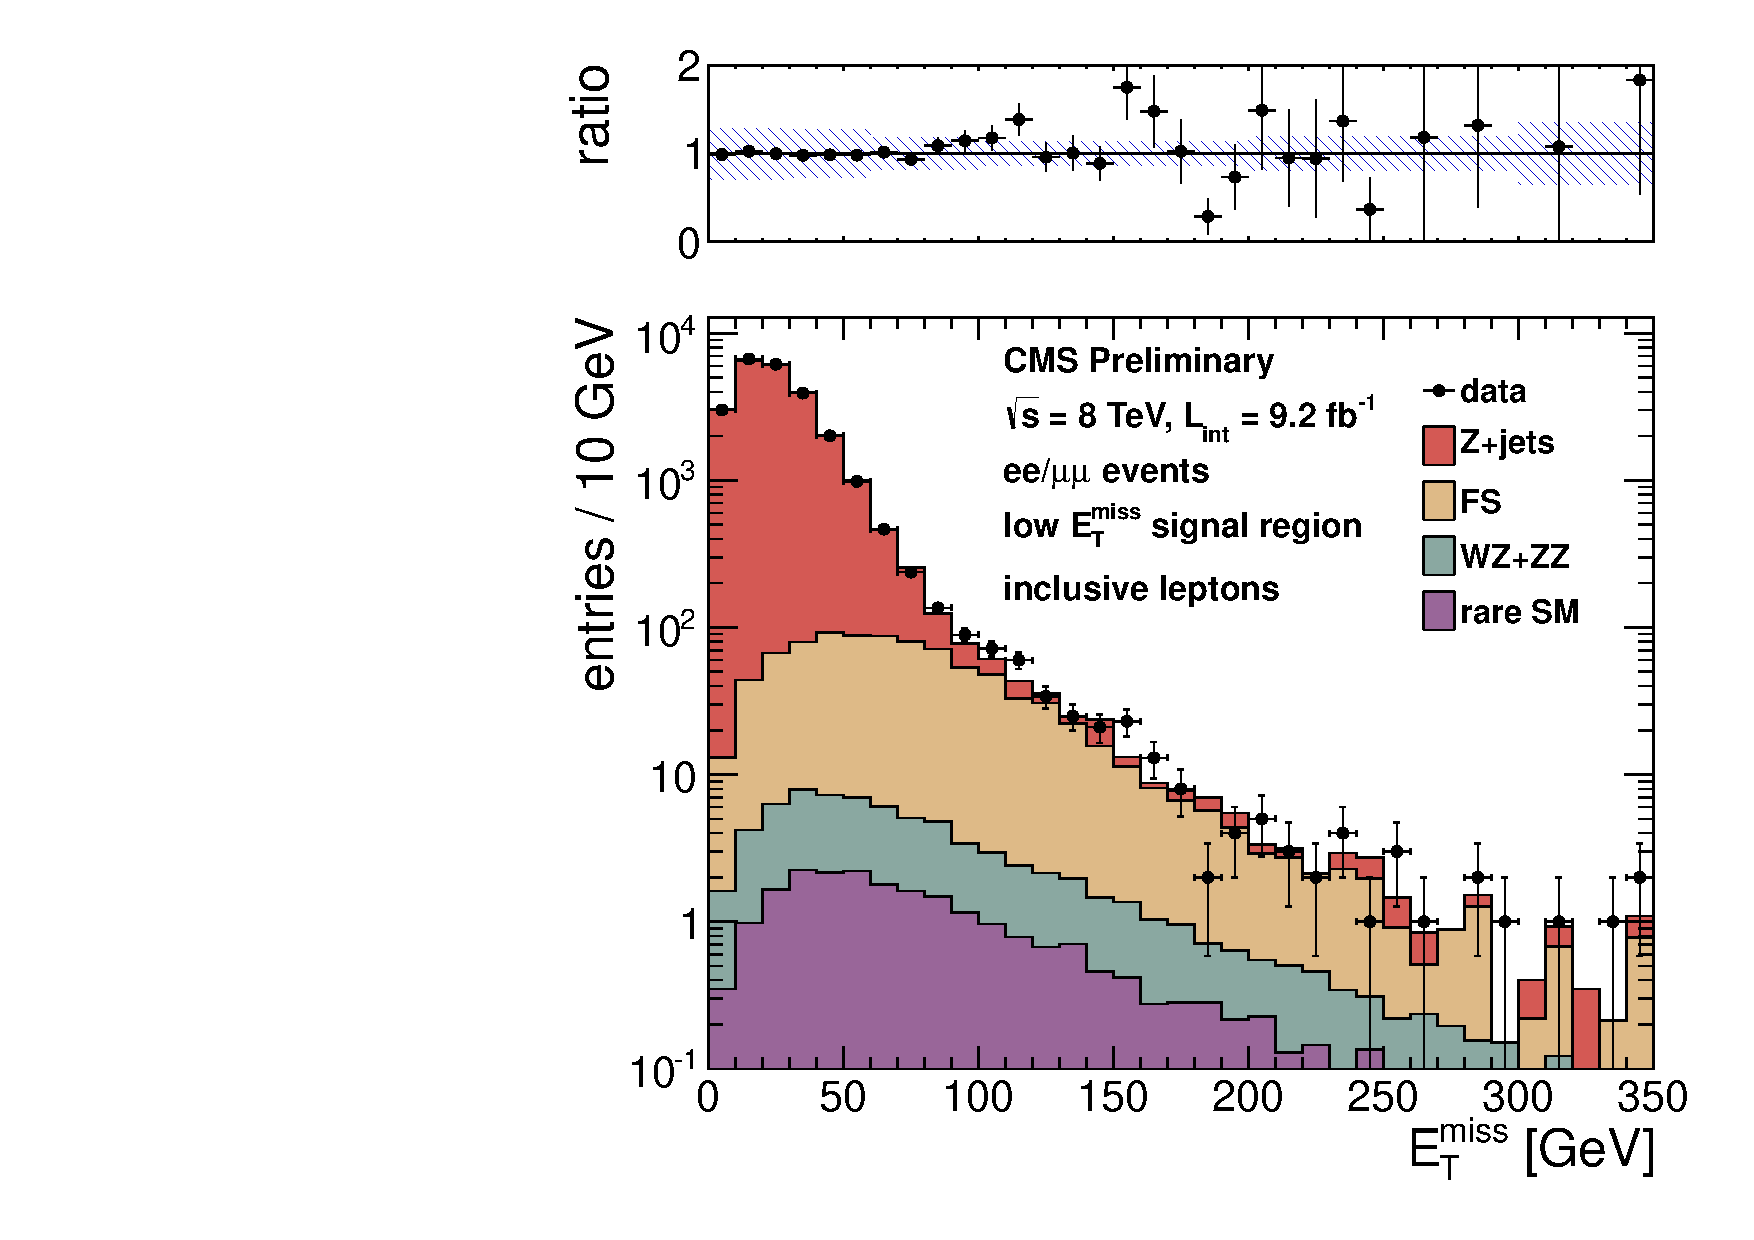
\includegraphics[width=0.45\textwidth]{plots/edge_pfmet_pt40_lowMet_all.pdf}
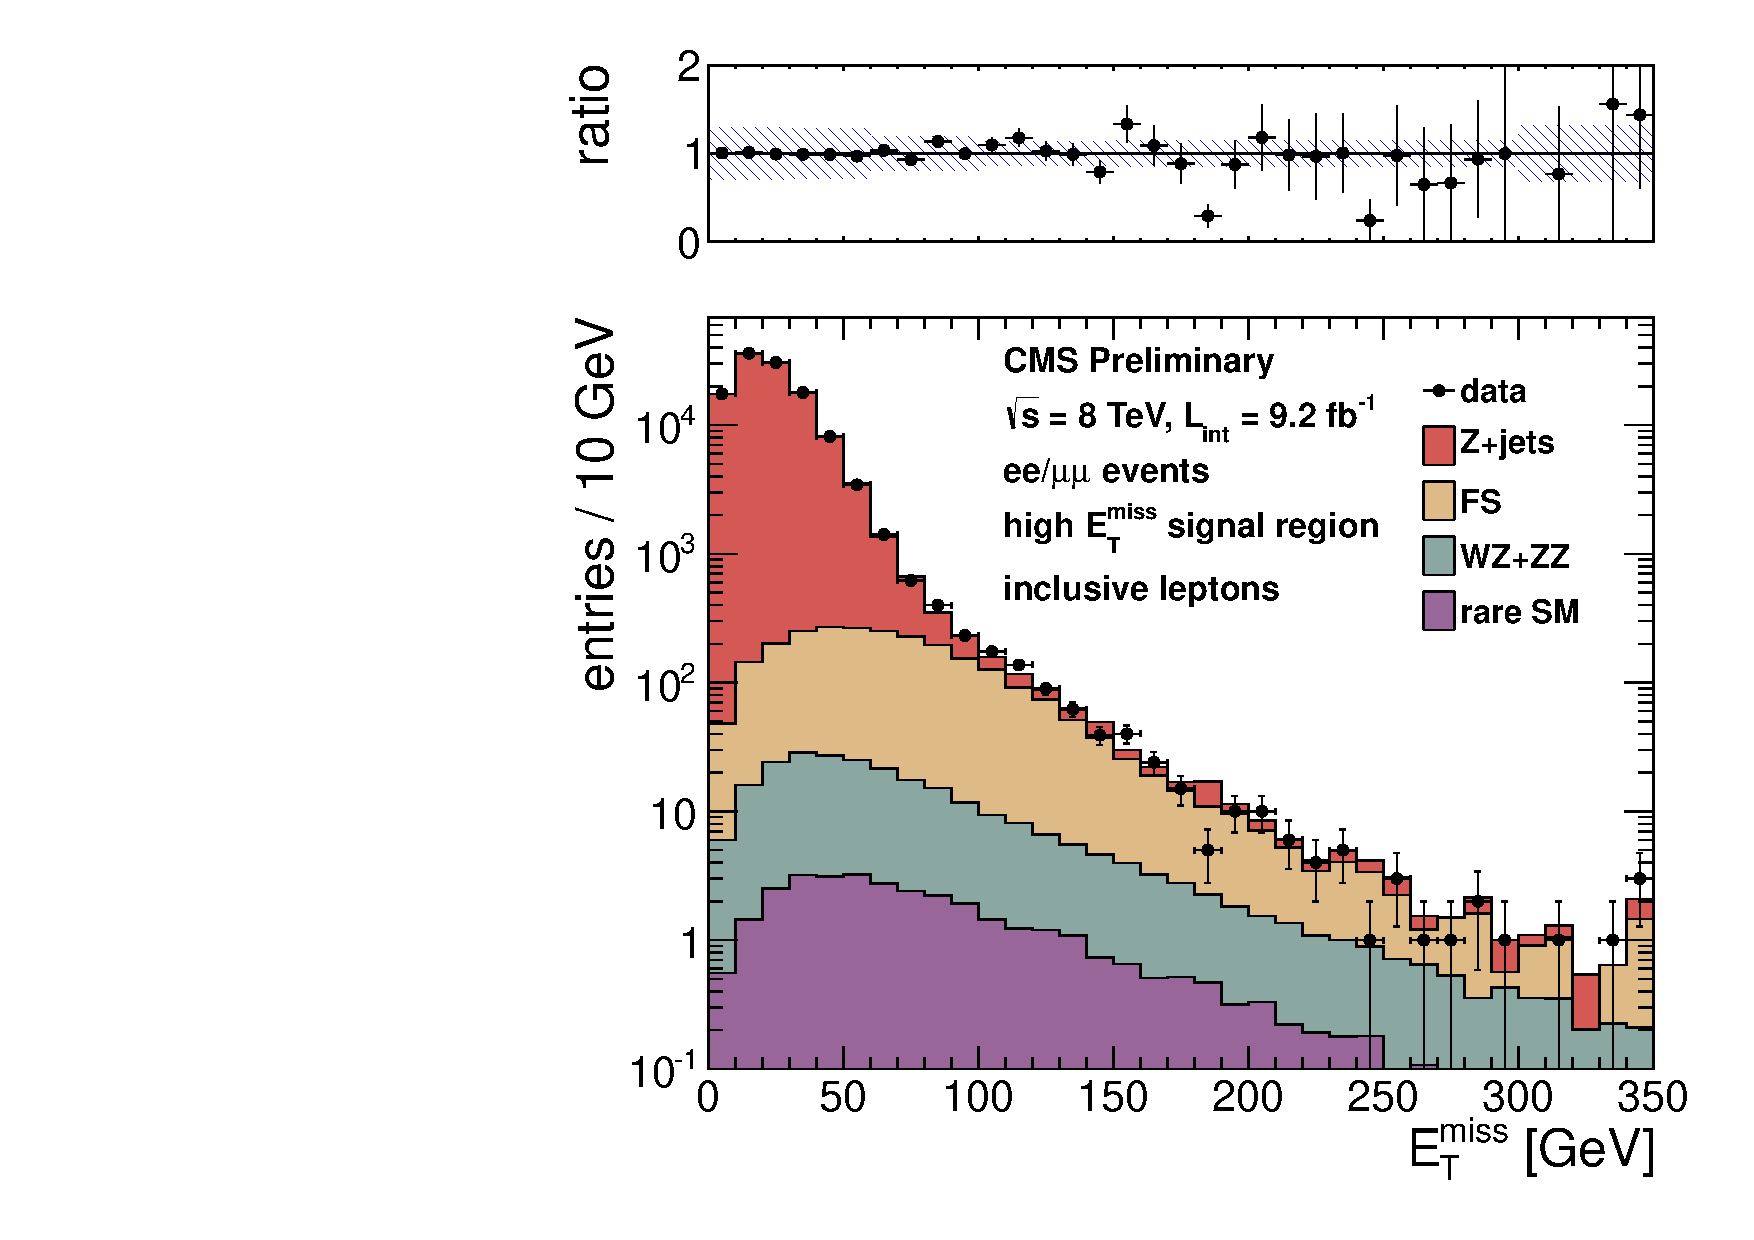
\includegraphics[width=0.45\textwidth]{plots/edge_pfmet_pt40_highMet_all.pdf}
%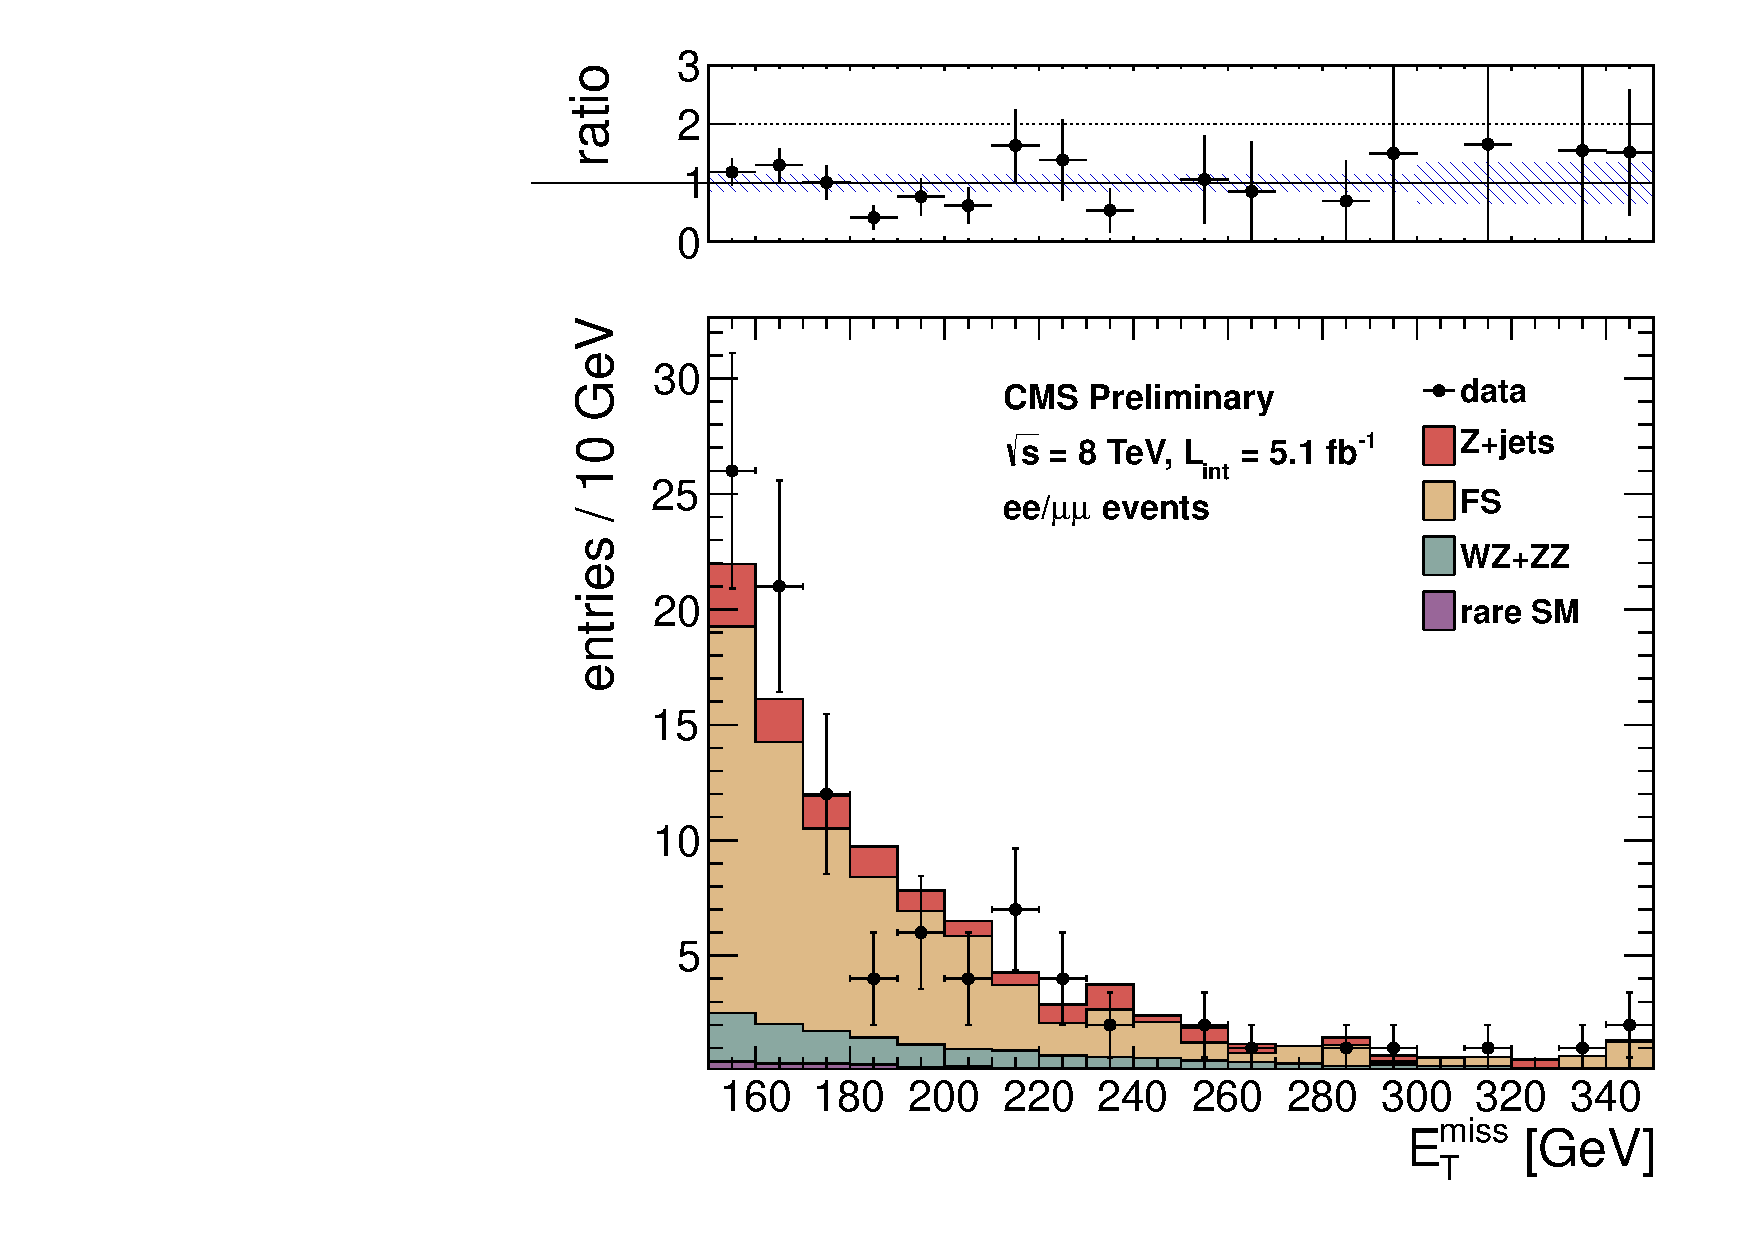
\includegraphics[width=0.48\textwidth]{plots/pfmet_pt40_2012AB_highMet_all_linear.pdf}
\end{tabular}
\caption{\footnotesize {\bf Results of for the low \MET\ (left) and high \MET\ (right) signal regions with the inclusive lepton selection.}
The observed \MET\ distribution (black points) is compared with the sum of the predicted \MET\
distributions from \zjets, flavor-symmetric backgrounds, WZ+ZZ backgrounds, and rare SM backgrounds. 
The ratio of observed to predicted yields in each bin is
indicated. The error bars indicate the statistical uncertainty in the data and the shaded band indicates the total background uncertainty.
\label{fig:results_inclusive}
}
\end{center}
\end{figure}

\begin{table}[htb]
\begin{center}
\footnotesize
\caption{\label{tab:results_inclusive}\footnotesize {\bf Results for the low \MET\ signal region (top table) and high \MET\ signal region (bottom table) with the inclusive lepton selection.} 
The total background is the sum of the \zjets\ background predicted from
the \MET\ templates method (\zjets\ bkg), the flavor-symmetric background predicted from e$\mu$ events (FS bkg), the WZ and ZZ backgrounds predicted from MC
(WZ bkg and ZZ bkg) and the rare SM backgrounds. All uncertainties include both the statistical and systematic components. The Gaussian significance of the deviation between the data 
and total background is indicated for signal regions with at least 20 observed events. }
\begin{tabular}{l|c|c|c|c|c|c}

\hline
\hline

\begin{comment}
Using pfmet out-of-the-box
NEED TO RE-EVALUATE K!!!!!!!!!!!!!!!!!
Using pT > 40 GeV jets, low MET signal region
WZ/ZZ selection : ((((((leptype==0 && (ee==1 || isdata==0))||(leptype==1 && (mm==1 || isdata==0)))&&(ngennu>0))&&(csc==0 && hbhe==1 && hcallaser==1 && ecaltp==1 && trkfail==1 && eebadsc==1 && hbhenew==1))&&(dilmass>81 && dilmass<101))&&(lep1.pt()>20.0 && lep2.pt()>20.0))&&(njets40>=3)
WZ/ZZ weight    : weight * 9.2 * vtxweight * trgeff
Opening ../output/V00-01-04/babylooper_edge_data_ALL_53X_PhotonStitchedTemplate_pfmet_pt40_lowMet.root
B-veto?   0
K         0.14
ee+mm channels: scale em yield by 0.99
Yields in 0-60 GeV region
data   : 22782
gjets  : 23299
OF     : 350.242
WZ     : 22.2641
ZZ     : 2.36791
Rare   : 9.60548
Scaling gjets by : 0.961309
SF events 23999
OF events 5826

ee/#mu#mu events
\end{comment}

                      &   \MET\ $>$ 0 GeV   &  \MET\ $>$ 30 GeV   &  \MET\ $>$ 60 GeV   & \MET\ $>$ 100 GeV   & \MET\ $>$ 150 GeV   & \MET\ $>$ 300 GeV  \\
\hline
        \zjets\ bkg   &  23071 $\pm$ 6922   &   7456 $\pm$ 2238   &     673 $\pm$ 203   &   49.9 $\pm$ 16.4   &    10.4 $\pm$ 3.6   &     1.0 $\pm$ 0.6  \\
             FS bkg   &     807 $\pm$ 126   &     695 $\pm$ 108   &      457 $\pm$ 71   &      184 $\pm$ 29   &    45.6 $\pm$ 7.5   &     1.5 $\pm$ 0.5  \\
             WZ bkg   &   43.5 $\pm$ 30.5   &   35.1 $\pm$ 24.6   &   21.3 $\pm$ 14.9   &    10.0 $\pm$ 7.1   &     4.4 $\pm$ 3.2   &     0.4 $\pm$ 0.4  \\
             ZZ bkg   &     7.8 $\pm$ 3.9   &     7.0 $\pm$ 3.6   &     5.4 $\pm$ 2.8   &     3.3 $\pm$ 1.8   &     1.7 $\pm$ 1.1   &     0.2 $\pm$ 0.2  \\
        rare SM bkg   &   22.0 $\pm$ 11.0   &    19.0 $\pm$ 9.6   &    12.4 $\pm$ 6.3   &     6.3 $\pm$ 3.3   &     2.8 $\pm$ 1.6   &     0.3 $\pm$ 0.3  \\
\hline
          total bkg   &  23951 $\pm$ 6924   &   8213 $\pm$ 2241   &    1169 $\pm$ 216   & {\bf     253 $\pm$ 34 }  &    64.8 $\pm$ 9.1   &     3.5 $\pm$ 1.0  \\
               data   &             23999   &              8134   &              1217   & {\bf          288 }      &                76   &                 4  \\
       significance   &       0.0$\sigma$   &      -0.0$\sigma$   &       0.2$\sigma$   & {\bf      0.9$\sigma$ }  &       0.9$\sigma$   &                    \\
\hline
\hline

\begin{comment}
Using pfmet out-of-the-box
NEED TO RE-EVALUATE K!!!!!!!!!!!!!!!!!
Using pT > 40 GeV jets, high MET signal region
WZ/ZZ selection : (((((((leptype==0 && (ee==1 || isdata==0))||(leptype==1 && (mm==1 || isdata==0)))&&(ngennu>0))&&(csc==0 && hbhe==1 && hcallaser==1 && ecaltp==1 && trkfail==1 && eebadsc==1 && hbhenew==1))&&(dilmass>81 && dilmass<101))&&(lep1.pt()>20.0 && lep2.pt()>20.0))&&(njets40>=2))&&(ht40>=100.0)
WZ/ZZ weight    : weight * 9.2 * vtxweight * trgeff
Opening ../output/V00-01-04/babylooper_edge_data_ALL_53X_PhotonStitchedTemplate_pfmet_pt40_highMet.root
B-veto?   0
K         0.14
ee+mm channels: scale em yield by 0.99
Yields in 0-60 GeV region
data   : 113677
gjets  : 115027
OF     : 1054.05
WZ     : 100.866
ZZ     : 11.955
Rare   : 14.0179
Scaling gjets by : 0.978
SF events 116978
OF events 16270

ee/#mu#mu events
\end{comment}

                      &   \MET\ $>$ 0 GeV   &  \MET\ $>$ 30 GeV   &  \MET\ $>$ 60 GeV   & \MET\ $>$ 100 GeV   & \MET\ $>$ 150 GeV   & \MET\ $>$ 300 GeV  \\
\hline
        \zjets\ bkg   &114401 $\pm$ 34322   &  30966 $\pm$ 9291   &    1905 $\pm$ 573   &      120 $\pm$ 38   &    26.2 $\pm$ 8.9   &     1.4 $\pm$ 0.7  \\
             FS bkg   &    2255 $\pm$ 350   &    1908 $\pm$ 296   &    1201 $\pm$ 187   &      436 $\pm$ 68   &   90.0 $\pm$ 14.4   &     2.9 $\pm$ 0.8  \\
             WZ bkg   & 182.7 $\pm$ 127.9   & 144.7 $\pm$ 101.3   &   81.8 $\pm$ 57.3   &   35.2 $\pm$ 24.7   &    13.9 $\pm$ 9.9   &     1.3 $\pm$ 1.3  \\
             ZZ bkg   &   35.9 $\pm$ 18.0   &   32.3 $\pm$ 16.2   &   23.9 $\pm$ 12.0   &    14.0 $\pm$ 7.1   &     6.7 $\pm$ 3.6   &     0.8 $\pm$ 0.8  \\
        rare SM bkg   &   33.5 $\pm$ 16.8   &   29.0 $\pm$ 14.6   &    19.5 $\pm$ 9.8   &    10.2 $\pm$ 5.2   &     4.5 $\pm$ 2.5   &     0.5 $\pm$ 0.5  \\
\hline
          total bkg   &116908 $\pm$ 34324   &  33080 $\pm$ 9296   &    3231 $\pm$ 605   &      616 $\pm$ 82   & {\bf     141 $\pm$ 20 }  &     6.9 $\pm$ 1.9  \\
               data   &            116978   &             32796   &              3301   &               635   & {\bf              133 }  &                 5  \\
       significance   &       0.0$\sigma$   &      -0.0$\sigma$   &       0.1$\sigma$   &       0.2$\sigma$   & {\bf     -0.4$\sigma$ }  &                    \\

\hline
\hline

\end{tabular}
\end{center}
\end{table}

\clearpage


\begin{figure}[!h]
\begin{center}
\begin{tabular}{cc}
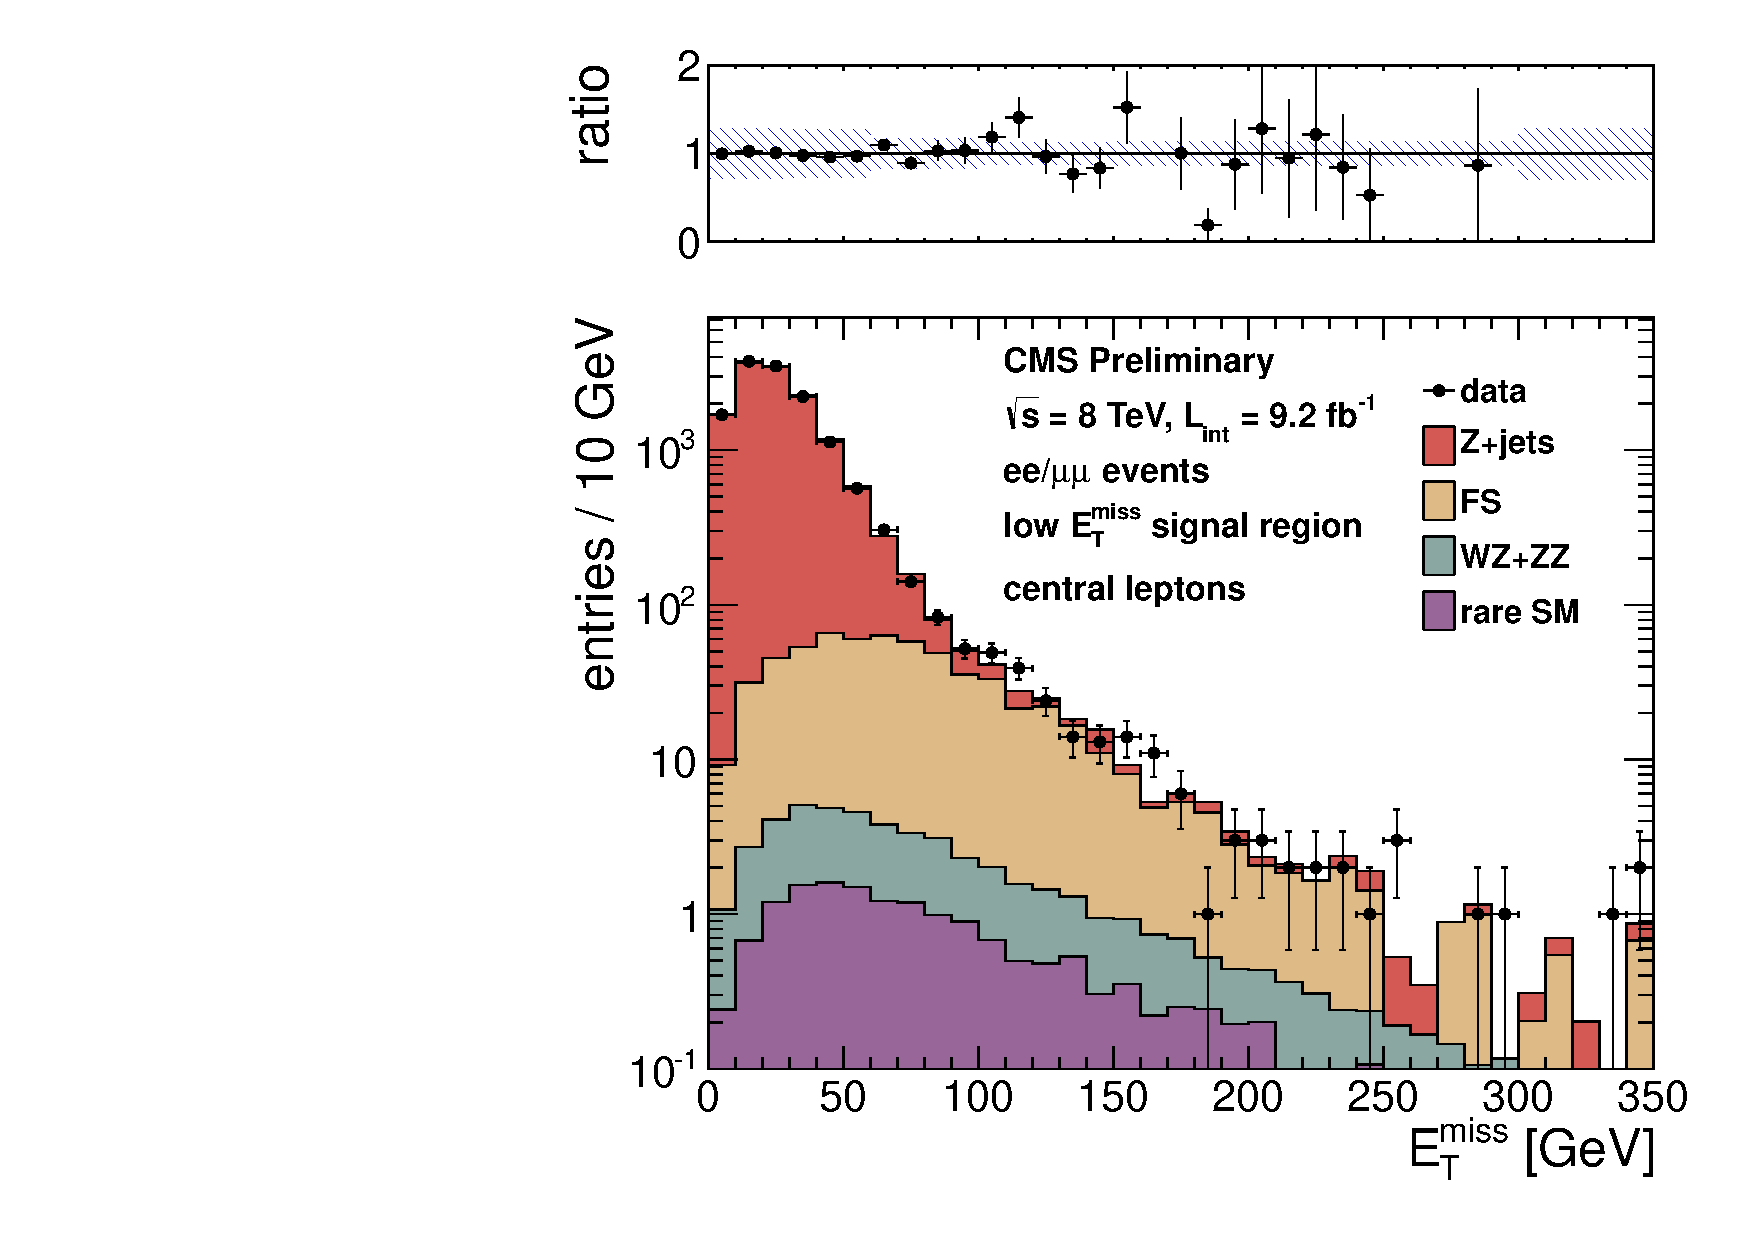
\includegraphics[width=0.45\textwidth]{plots/edge_pfmet_pt40_lowMet_central_all.pdf}
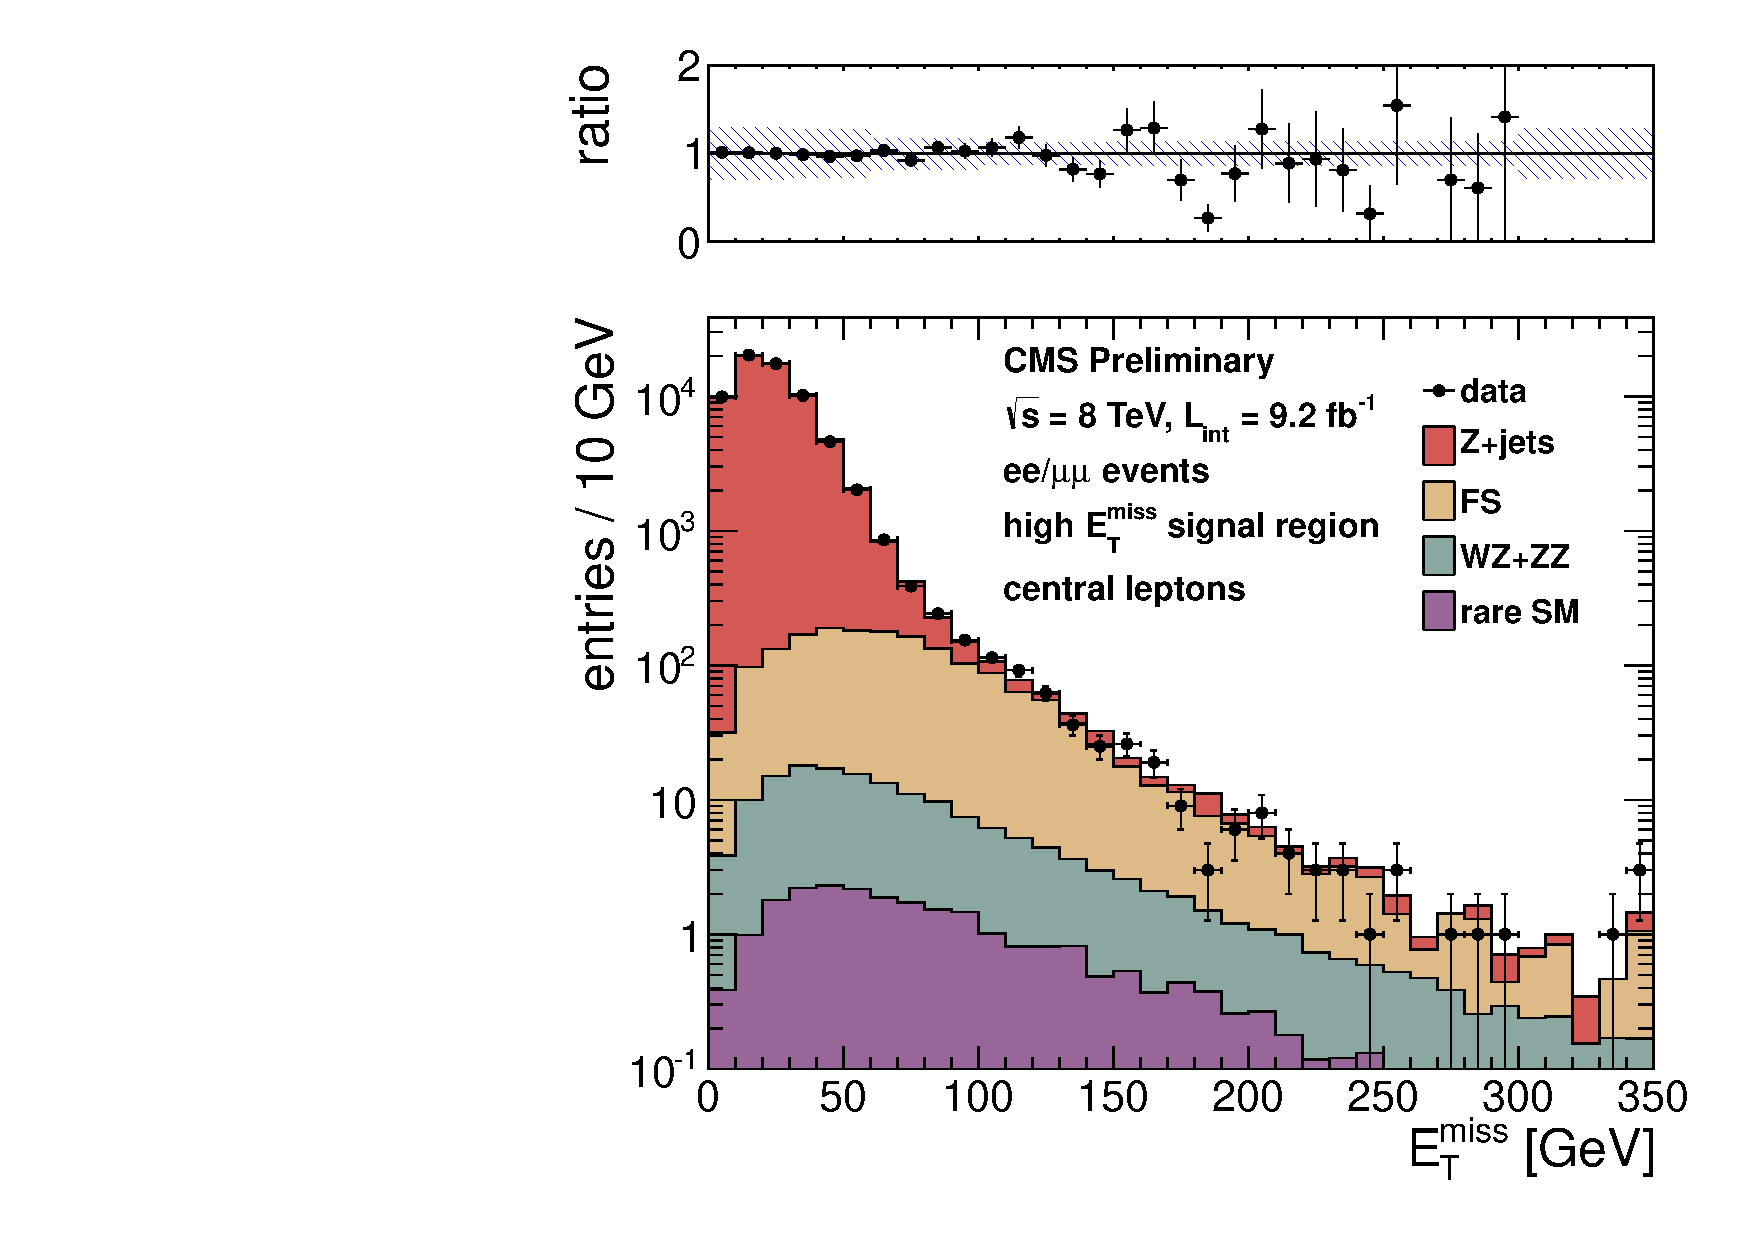
\includegraphics[width=0.45\textwidth]{plots/edge_pfmet_pt40_highMet_central_all.pdf}
%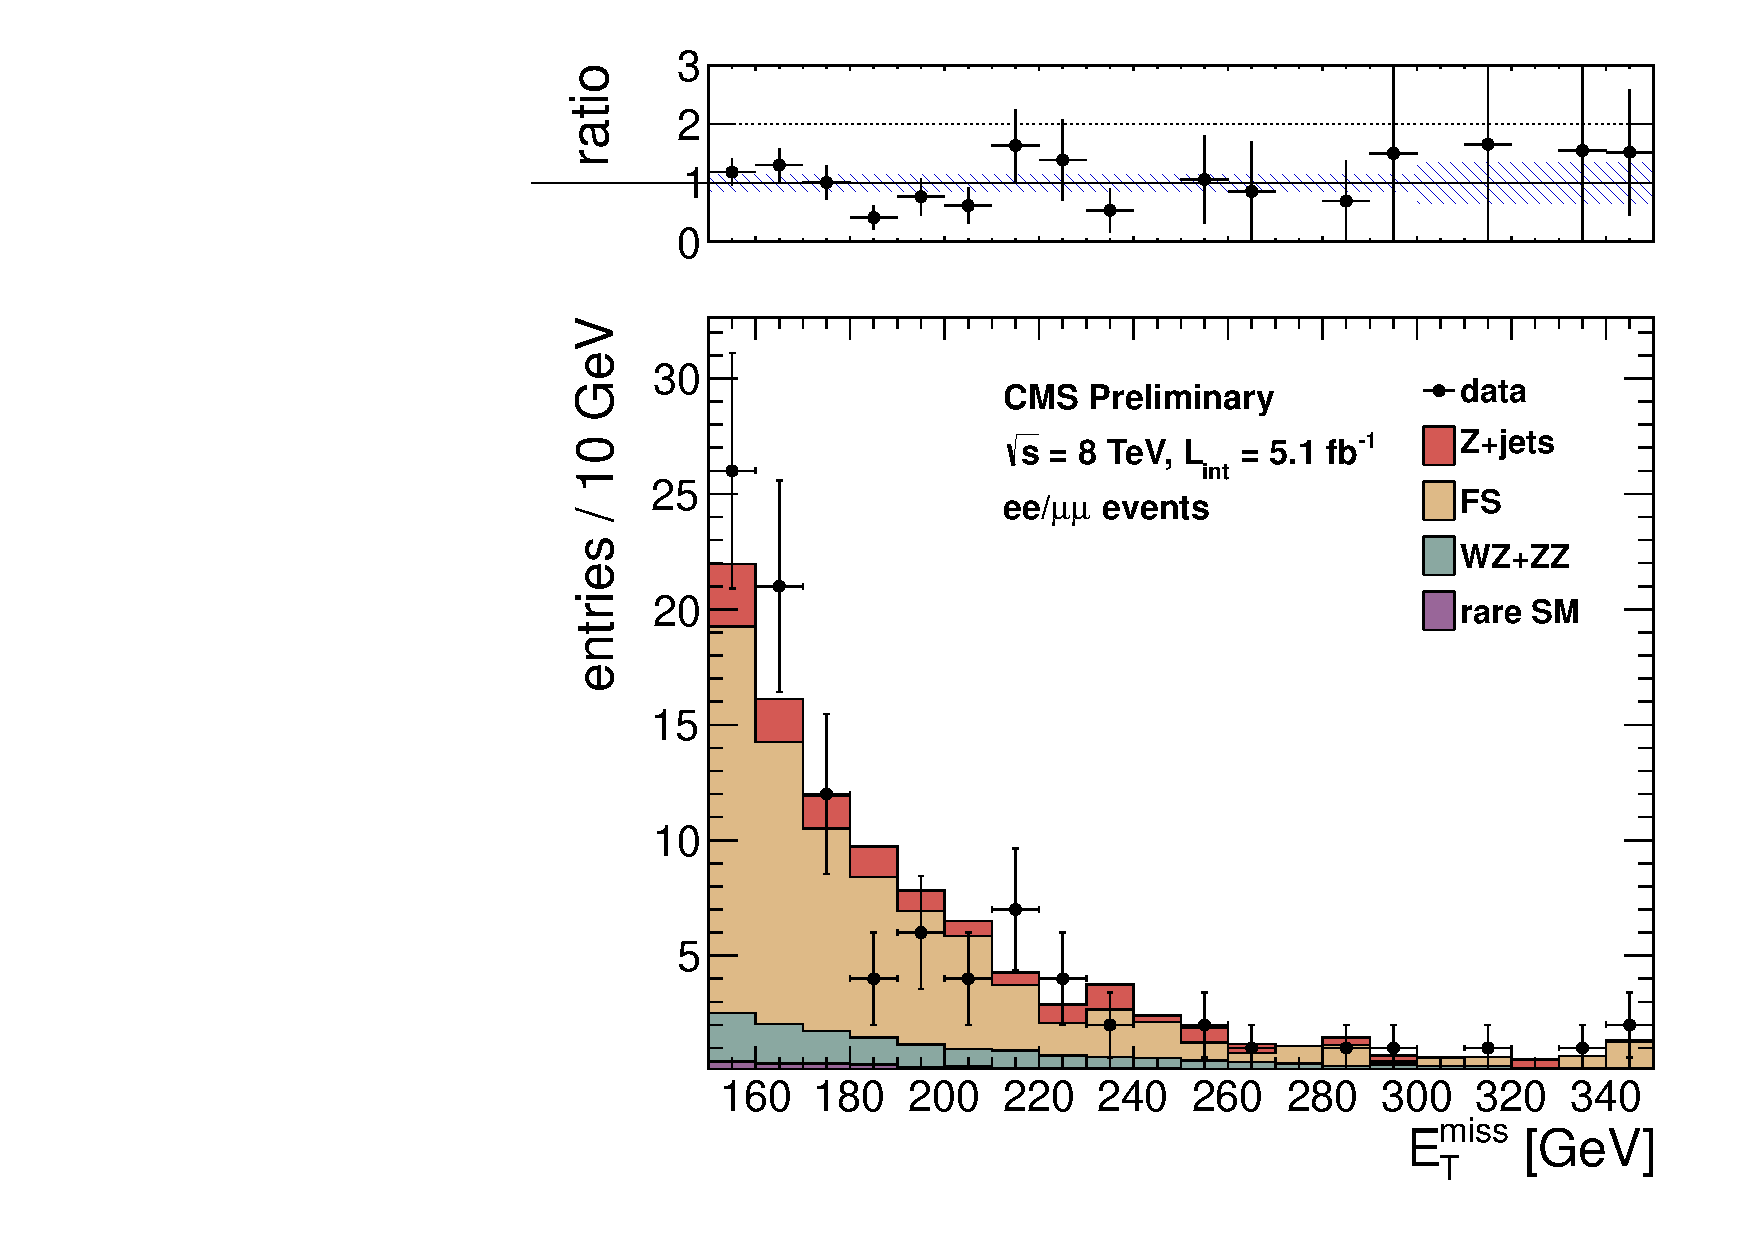
\includegraphics[width=0.48\textwidth]{plots/pfmet_pt40_2012AB_highMet_all_linear.pdf}
\end{tabular}
\caption{\footnotesize {\bf Results of for the low \MET\ (left) and high \MET\ (right) signal regions with the central lepton selection.}
The observed \MET\ distribution (black points) is compared with the sum of the predicted \MET\
distributions from \zjets, flavor-symmetric backgrounds, WZ+ZZ backgrounds, and rare SM backgrounds. 
The ratio of observed to predicted yields in each bin is
indicated. The error bars indicate the statistical uncertainty in the data and the shaded band indicates the total background uncertainty.
\label{fig:results_central}
}
\end{center}
\end{figure}

\begin{table}[htb]
\begin{center}
\footnotesize
\caption{\label{tab:results_central}\footnotesize {\bf Results for the low \MET\ signal region (top table) and high \MET\ signal region (bottom table) with the central lepton selection.} 
The total background is the sum of the \zjets\ background predicted from
the \MET\ templates method (\zjets\ bkg), the flavor-symmetric background predicted from e$\mu$ events (FS bkg), the WZ and ZZ backgrounds predicted from MC
(WZ bkg and ZZ bkg) and the rare SM backgrounds. All uncertainties include both the statistical and systematic components. The Gaussian significance of the deviation between the data 
and total background is indicated for signal regions with at least 20 observed events. }
\begin{tabular}{l|c|c|c|c|c|c}

\hline
\hline

\begin{comment}
Using pfmet out-of-the-box
NEED TO RE-EVALUATE K!!!!!!!!!!!!!!!!!
Using pT > 40 GeV jets, low MET signal region, central leptons
WZ/ZZ selection : (((((((leptype==0 && (ee==1 || isdata==0))||(leptype==1 && (mm==1 || isdata==0)))&&(ngennu>0))&&(csc==0 && hbhe==1 && hcallaser==1 && ecaltp==1 && trkfail==1 && eebadsc==1 && hbhenew==1))&&(dilmass>81 && dilmass<101))&&(lep1.pt()>20.0 && lep2.pt()>20.0))&&(njets40>=3))&&(abs(lep1.eta()) < 1.4 && abs(lep2.eta()) < 1.4)
WZ/ZZ weight    : weight * 9.2 * vtxweight * trgeff
Opening ../output/V00-01-04/babylooper_edge_data_ALL_53X_PhotonStitchedTemplate_pfmet_pt40_lowMet_central.root
B-veto?   0
K         0.15
ee+mm channels: scale em yield by 0.99
Yields in 0-60 GeV region
data   : 12858
gjets  : 13220.3
OF     : 242.649
WZ     : 14.1734
ZZ     : 1.45279
Rare   : 6.75969
Scaling gjets by : 0.952549
SF events 13631
OF events 3806

ee/#mu#mu events
\end{comment}

                      &   \MET\ $>$ 0 GeV   &  \MET\ $>$ 30 GeV   &  \MET\ $>$ 60 GeV   & \MET\ $>$ 100 GeV   & \MET\ $>$ 150 GeV   & \MET\ $>$ 300 GeV  \\
\hline
        \zjets\ bkg   &  12984 $\pm$ 3896   &   4242 $\pm$ 1273   &     391 $\pm$ 118   &    29.6 $\pm$ 9.7   &     6.3 $\pm$ 2.2   &     0.6 $\pm$ 0.4  \\
             FS bkg   &      565 $\pm$ 83   &      487 $\pm$ 72   &      323 $\pm$ 48   &      129 $\pm$ 19   &    32.5 $\pm$ 5.2   &     1.2 $\pm$ 0.5  \\
             WZ bkg   &   28.1 $\pm$ 19.7   &   22.7 $\pm$ 15.9   &    13.9 $\pm$ 9.8   &     6.8 $\pm$ 4.9   &     3.1 $\pm$ 2.4   &     0.4 $\pm$ 0.4  \\
             ZZ bkg   &     4.8 $\pm$ 2.5   &     4.4 $\pm$ 2.3   &     3.3 $\pm$ 1.8   &     2.1 $\pm$ 1.2   &     1.1 $\pm$ 0.8   &     0.1 $\pm$ 0.1  \\
        rare SM bkg   &    15.8 $\pm$ 8.0   &    13.7 $\pm$ 6.9   &     9.0 $\pm$ 4.6   &     4.8 $\pm$ 2.5   &     2.3 $\pm$ 1.4   &     0.3 $\pm$ 0.3  \\
\hline
          total bkg   &  13598 $\pm$ 3897   &   4770 $\pm$ 1275   &     740 $\pm$ 128   &{\bf      173 $\pm$ 22}   &    45.2 $\pm$ 6.3   &     2.6 $\pm$ 0.7  \\
               data   &             13631   &              4688   &               773   &{\bf               192}   &                53   &                 3  \\
       significance   &       0.0$\sigma$   &      -0.1$\sigma$   &       0.3$\sigma$   &{\bf       0.7$\sigma$}   &       0.8$\sigma$   &                    \\
\hline
\hline

\begin{comment}
Using pfmet out-of-the-box
NEED TO RE-EVALUATE K!!!!!!!!!!!!!!!!!
Using pT > 40 GeV jets, high MET signal region, central leptons
WZ/ZZ selection : ((((((((leptype==0 && (ee==1 || isdata==0))||(leptype==1 && (mm==1 || isdata==0)))&&(ngennu>0))&&(csc==0 && hbhe==1 && hcallaser==1 && ecaltp==1 && trkfail==1 && eebadsc==1 && hbhenew==1))&&(dilmass>81 && dilmass<101))&&(lep1.pt()>20.0 && lep2.pt()>20.0))&&(njets40>=2))&&(ht40>=100.0))&&(abs(lep1.eta()) < 1.4 && abs(lep2.eta()) < 1.4)
WZ/ZZ weight    : weight * 9.2 * vtxweight * trgeff
Opening ../output/V00-01-04/babylooper_edge_data_ALL_53X_PhotonStitchedTemplate_pfmet_pt40_highMet_central.root
B-veto?   0
K         0.15
ee+mm channels: scale em yield by 0.99
Yields in 0-60 GeV region
data   : 64459
gjets  : 65372.5
OF     : 722.898
WZ     : 62.6465
ZZ     : 6.86106
Rare   : 9.85893
Scaling gjets by : 0.973755
SF events 66521
OF events 10593

ee/#mu#mu events
\end{comment}

                      &   \MET\ $>$ 0 GeV   &  \MET\ $>$ 30 GeV   &  \MET\ $>$ 60 GeV   & \MET\ $>$ 100 GeV   & \MET\ $>$ 150 GeV   & \MET\ $>$ 300 GeV  \\
\hline
        \zjets\ bkg   & 64775 $\pm$ 19433   &  17697 $\pm$ 5310   &    1118 $\pm$ 336   &   71.8 $\pm$ 22.3   &    15.8 $\pm$ 5.3   &     0.8 $\pm$ 0.4  \\
             FS bkg   &    1573 $\pm$ 231   &    1341 $\pm$ 197   &     850 $\pm$ 125   &      313 $\pm$ 46   &   66.5 $\pm$ 10.2   &     2.2 $\pm$ 0.7  \\
             WZ bkg   &  115.0 $\pm$ 80.5   &   91.3 $\pm$ 64.0   &   52.4 $\pm$ 36.7   &   23.3 $\pm$ 16.4   &     9.4 $\pm$ 6.7   &     1.0 $\pm$ 1.0  \\
             ZZ bkg   &   21.7 $\pm$ 10.9   &    19.7 $\pm$ 9.9   &    14.8 $\pm$ 7.5   &     8.8 $\pm$ 4.5   &     4.3 $\pm$ 2.4   &     0.5 $\pm$ 0.5  \\
        rare SM bkg   &   23.9 $\pm$ 12.0   &   20.8 $\pm$ 10.4   &    14.1 $\pm$ 7.1   &     7.5 $\pm$ 3.9   &     3.6 $\pm$ 2.1   &     0.5 $\pm$ 0.5  \\
\hline
          total bkg   & 66508 $\pm$ 19435   &  19170 $\pm$ 5314   &    2049 $\pm$ 360   &      424 $\pm$ 54   &{\bf   99.6 $\pm$ 13.7}   &     5.1 $\pm$ 1.4  \\
               data   &             66521   &             18841   &              2062   &               421   &{\bf                92}   &                 4  \\
       significance   &       0.0$\sigma$   &      -0.1$\sigma$   &       0.0$\sigma$   &      -0.1$\sigma$   &{\bf      -0.5$\sigma$}   &                    \\
\hline
\hline

\end{tabular}
\end{center}
\end{table}

\clearpage


\subsection{Extrapolation to Low Mass to Estimate the $\gamma^*/Z$ Contribution}

Given a prediction for the Z background in the Z mass window, we can extrapolate to estimate the low mass $\gamma^*$/Z contribution.
We extract the ratio \rlowin\ of low-mass  to on-shell Z events from data,
correcting for the contribution from flavor-symmetric backgrounds, according to:

\begin{equation}
R_{low/in} = (N_{SF}^{low}-N_{OF}^{low})/(N_{SF}^{in}-N_{OF}^{in}).
\end{equation}

Here SF and OF refer to the same-flavor and opposite-flavor data yields in the ``low'' ($20<m_{\ell\ell}<70$ GeV) and ``in'' 
($81<m_{\ell\ell}<101$ GeV) dilepton mass regions. To predict the low-mass $\gamma^*$/Z contribution, we scale the total predicted
Z background by this quantity. The measurement of \rlowin\ is summarized in App.~\ref{app:R}; to summarize, we find \rlowin$=0.07\pm0.02$.

To predict the low-mass $\gamma*$/Z background, we start with the prediction for the total Z background in the on-Z regions for the four signal
regions (see the bold numbers from Tables~\ref{tab:results_inclusive} and \ref{tab:results_central}). Here the total Z background is the sum of \zjets,
WZ, ZZ, and rare SM backgrounds. This background is then scaled by \rlowin\ to predict the $\gamma*$/Z contribution to the low-mass region of the
four signal regions. The results are summarized in Table~\ref{tab:results}.

%We find the following results for the first 5.1 fb$^{-1}$. For the low \MET\ signal region, the total predicted Z background in the Z mass region is $39\pm9.6$ 
%(sum of the \zjets, WZ+ZZ, and rare SM backgrounds from Table~\ref{tab:results_lowmet}, \MET\ $>$ 100 GeV region), 
%resulting in a $\gamma^*$/Z prediction of $3.1\pm1.1$ events. 
%For the high \MET\ signal region, the total predicted Z background in the Z mass region is $30\pm8.1$ 
%(sum of the \zjets, WZ+ZZ, and rare SM backgrounds from Table~\ref{tab:results_highmet}, \MET\ $>$ 150 GeV region), 
%resulting in a $\gamma^*$/Z prediction of $3.8\pm1.4$ events. 

%We find the following results for the full 9.2 fb$^{-1}$. For the low \MET\ signal region, the total predicted Z background in the Z mass region is $68\pm17$ 
%(sum of the \zjets, WZ+ZZ, and rare SM backgrounds from Table~\ref{tab:results_edgefull}, \MET\ $>$ 100 GeV region), 
%resulting in a $\gamma^*$/Z prediction of $5.4\pm1.9$ events. 
%For the high \MET\ signal region, the total predicted Z background in the Z mass region is $60\pm16$ 
%(sum of the \zjets, WZ+ZZ, and rare SM backgrounds from Table~\ref{tab:results_edgefull}, \MET\ $>$ 150 GeV region), 
%resulting in a $\gamma^*$/Z prediction of $7.9\pm2.7$ events. 

\section{Summary of Results}
\label{sec:templates_summary}

As summary of the results in presented in Table~\ref{tab:results}. The observed data yields in the on-Z regions for the four signal regions
(low-\MET\ and high-\MET, inclusive and central leptons) are in good agreement with the predicted backgrounds.

\begin{table}[htb]
\begin{center}
\caption{\label{tab:results} Summary of results in the four signal regions.
The total observed yields in the on-Z regions (Total On-Z Yield) is compared to the total predicted background in the on-Z region (Total On-Z Bkg).
The total Z background (sum of \zjets, WZ, ZZ, and rare SM backgrounds) in the on-Z region is indicated (On-Z Z Bkg).
This Z background is scaled by \rlowin$=0.07 \pm 0.02$ to predict the $\gamma*$/Z contribution to the low-mass region ($\gamma*$/Z Bkg).
}
\begin{tabular}{l|c|c|c|c}

\hline
\hline
& Low-\MET\ (inclusive) & High-\MET\ (inclusive) & Low-\MET\ (central) & High-\MET\ (central)  \\
\hline              
Total On-Z Yield       & 288             & 133             &     192           &   92         \\
Total On-Z Bkg         & 253 $\pm$ 34    & 141 $\pm$ 20    &   173 $\pm$ 22    & 100 $\pm$ 14 \\
\hline
On-Z Z Bkg             & 70 $\pm$ 18     &  51 $\pm$ 14    &   43 $\pm$ 11     & 33 $\pm$ 9.1 \\
$\gamma*$/Z Bkg        & 4.9 $\pm$ 1.9   &  3.6 $\pm$ 1.4  &   3.0 $\pm$ 1.2   & 2.3 $\pm$0.9 \\
\hline
\hline

\end{tabular}
\end{center}
\end{table}

\clearpage


